\chapter{Directional Sound Separation}\label{ch:directional}
This chapter deals with directional filtering. In the beginning, the prerequisites 
for the filtering idea are presented. Afterwards, the actual filtering idea is 
shown and explained. In the end, the results are presented, and a conclusion is 
drawn.
\section{Concept}
Figure \ref{fig:2sources} shows a scenario where directional filtering could be 
used. Source 1 and Source 2 are both talking simultaneously. At the origin, two 
microphones, left (L) and right (R) are fixed and recording.

\begin{figure}[htp]
	\centering
	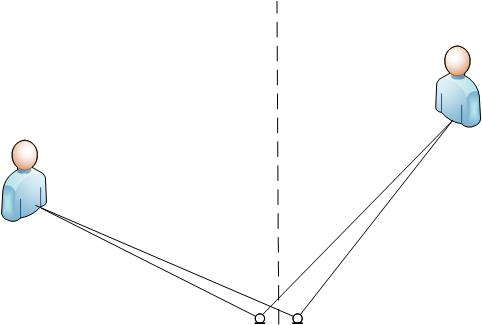
\includegraphics[width=0.65\textwidth]{Illustrations/2sources.jpg}
	\caption{Two Persons Talking}
	\label{fig:2sources}
\end{figure}

Due to the nature of the setup, the microphones will record  both the speakers.
However, both microphones record two persons talking. As a consequence, each 
microphone returns a soundwave containing two signals. The aim is to filter out one 
of them by only using the two soundwaves available.

In order to be able to do this, one assumption needs to be made. That is, that the 
angle at which each source is located, is known.

\begin{figure}[htp]
	\centering
	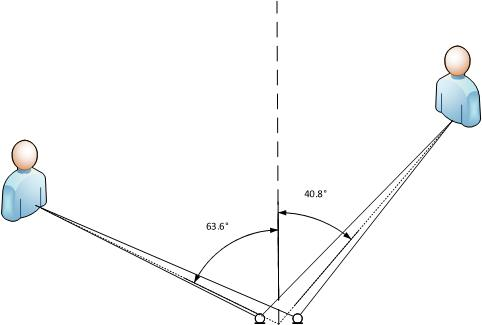
\includegraphics[width=0.67\textwidth]{Illustrations/2sourcesWangles.jpg}
	\caption{Two Persons Talking With Known Angles}
	\label{fig:2sourcesWangles}
\end{figure}

Figure \ref{fig:2sourcesWangles} represents the same scenario. However this time, 
the angles of the sound sources are known. The Sources and the Origin are 
represented with coordinates. This helps in determining the formulas that are 
needed in order to obtain the delay in samples.

\begin{figure}[htp]
	\centering
	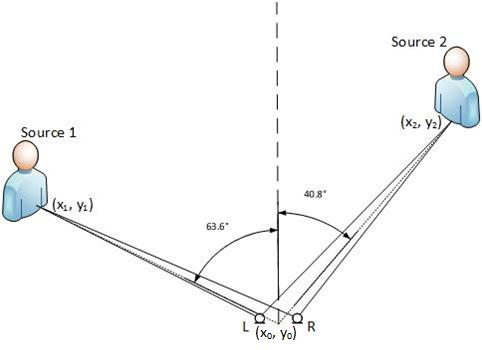
\includegraphics[width=0.67\textwidth]{Illustrations/2sourcesWanglesAndPossition.jpg}
	\caption{Two Persons Talking With Known Angles}
	\label{fig:2sourcesWanglesAndPossition}
\end{figure}

\newpage

Figure \ref{fig:zoomedin1} represents the delay between the two signals. One 
advantage is represented by the fact that, no matter the distance of the source, 
the delay between the signals is always the same. The delay in samples is only 
dependent on the distance between the mics. By knowing the angle, the sampling 
frequency and the speed of sound, the delay in samples can be determined. By 
increasing the distance between the microphones, greater accuracy could be 
obtained. However this would also result in a bigger difference in terms of signal 
gain. One signal would be significantly louder than the other to the point where 
filtering would not work.


\begin{figure}[htp]
	\centering
	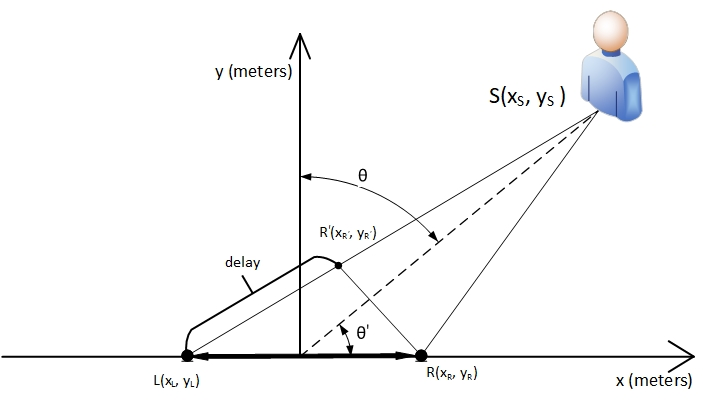
\includegraphics[width=0.65\textwidth]{Illustrations/delayDrawingForEquations.jpg}
	\caption{Delay}
	\label{fig:zoomedin1}
\end{figure}

\newpage
\section{Mathematical Solution}

Figure \ref{fig:zoomedin2} is a more detailed version of Figure \ref{fig:zoomedin1} 
in order to better understand and explain the mathematical proof of finding the 
delay in number of samples.

\begin{figure}[htp]
	\centering
	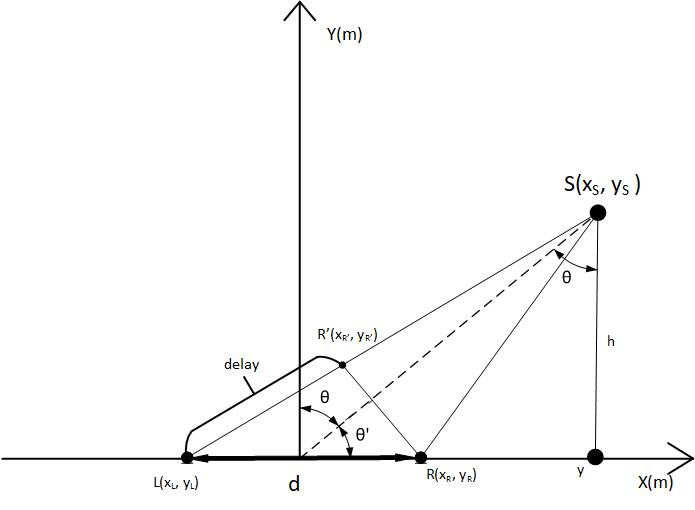
\includegraphics[width=1\textwidth]{Illustrations/mathematicalShit.jpg}
	\caption{Mathematical Interpretation}
	\label{fig:zoomedin2}
\end{figure}

Firstly, the distances SR and SL must be determined. This can be found by employing 
basic trigonometry. This is done by independently finding out the sides SA, AR and 
AL of the triangles $\triangle$SAL  and $\triangle$SAR. Distances SR' and SR are 
equal, based on the fact that angles $\angle$SRR' = $\angle$SR'R. Distance LR is 
denoted as "gap" and SL as "h" to make it easier to follow the equations. C is the 
center point between left and right microphones.
\begin{equation}
	AR = sin(\theta) \cdot CS  - \dfrac{gap}{2} 
\end{equation}

\begin{equation}
	AL = sin(\theta) \cdot CS + \dfrac{gap}{2}
\end{equation}

After the x-coordinates are determined, h is needed in order to calculate the y-
coordinates.

\begin{equation}
	h = cos(\theta) \cdot CS
\end{equation}

\newpage
Lastly, the sides SR and SL are determined.

\begin{equation}
	SR = \sqrt{h^2 + AR^2}
\end{equation}

\begin{equation}
	SL = \sqrt{h^2 + AL^2}
\end{equation}

Once the distances are known, the difference in distance between the signals can be 
found.

\begin{equation}
	delay = SL - SR
\end{equation}

At this moment, the delay is expressed in distance. By knowing the speed of sound 
(\(v_s\)), the amount of time it takes to travel that distance can be found.

\begin{equation}
	delayInTime = \frac{delay}{v_s}
\end{equation}

The time, can be converted in amount of samples by multiplying it by the sampling 
frequency.

\begin{equation}
	delayInSamples = delayInTime \cdot SamplingFrequncy
\end{equation}

There are 2 variables influencing the delay (the gap between microphones is 
set constant). Angle of where the source is placed at and the distance to it have 
to be measured with a help of sensors. To determine whether we need to measure both 
of them, we looked at how different angles and distances to the source affect the 
delay (see figure \ref{fig:anglesDistDelay}).

\begin{figure}[htp]
	\centering
	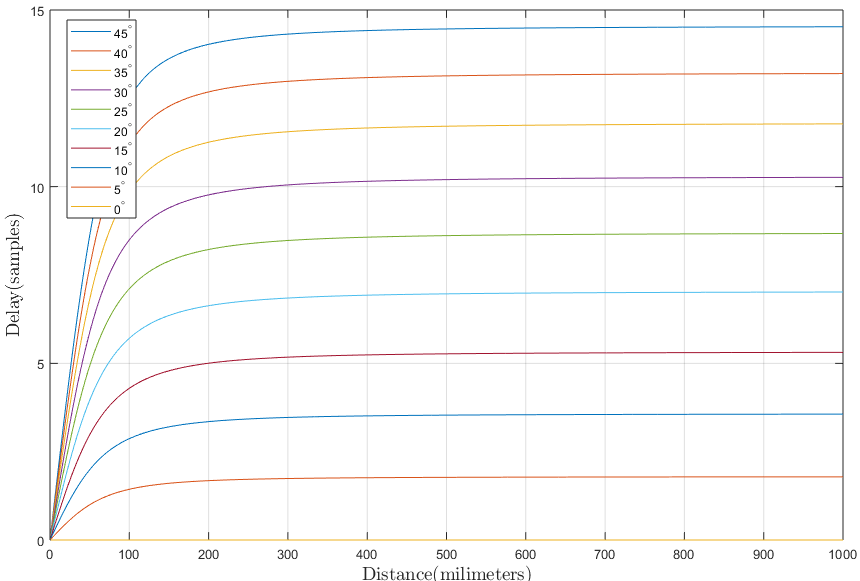
\includegraphics[width=0.75\textwidth]{Illustrations/distanceMatters.png}
	\caption{Angle and Distance Effects on Delay}
	\label{fig:anglesDistDelay}
\end{figure}

From the graph above we can see, that just after 30cm, distance stops affecting the 
delay significantly. Furthermore, since samples can only be integer numbers, we are 
rounding down delays in samples to the closest integer. Based on this finding, we 
have decided to set distance to 1 meter to simplify our calculations.

\newpage
\section{Filtering Idea}
With the angles of both sources known, one or the other source can be isolated. The 
only sound source considered in this project was human voice. Therefore, the aim is 
to separate the two voices, by only using the sound samples recorded by both 
microphones. The data recorded by each microphone, contains two separate human 
speeches. Figure \ref{fig:IdeaDiagram} explains the process. Afterwards, a more 
visual example will be discussed, aimed at better describing the procedure. 

\begin{figure}[htp]
	\centering
	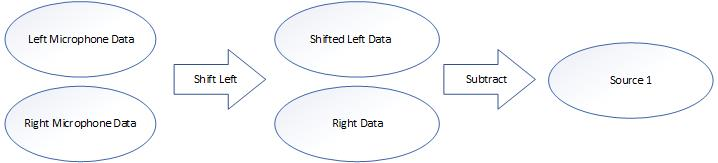
\includegraphics[width=1\textwidth]{Illustrations/IdeaDiagram.jpg}
	\caption{Idea diagram}
	\label{fig:IdeaDiagram}
\end{figure}

Both microphones record the same data. The only two differences, are the delay in 
time, and the gain difference. By shifting one recorded sample in order to match 
the other, and subtracting the signals, the matched data is eliminated. This means 
that by aligning one speech, and then subtracting, the other speech is separated 
and obtained.

\newpage

\section{Visual Example}
A visual example is explained below. Actual differences can even be seen on the 
waveforms themselves. The example is ideal, meaning there is no noise applied to 
the signals, and their purpose is to prove the idea.\\

To better understand the example the following notation is used to represent the 
amount of samples the signal has been shifted. 

\begin{align}
	Signal1(-389)
	\label{eq:signal1}
\end{align}
\begin{align}
	Signal2(254)
	\label{eq:signal2}
\end{align}

Signal1 in Equation \ref{eq:signal1} has been shifted to the left by 389 samples. 
Meaning that, if plotted, Signal1(-389) would be ahead of Signal1 by 389 samples.

Signal2 in Equation \ref{eq:signal2} has been shifted to the right by 254 samples. 
Meaning that, if plotted, Signal2(254) would be behind Signal2 by 254 samples.

\begin{figure}[htp]
	\centering
	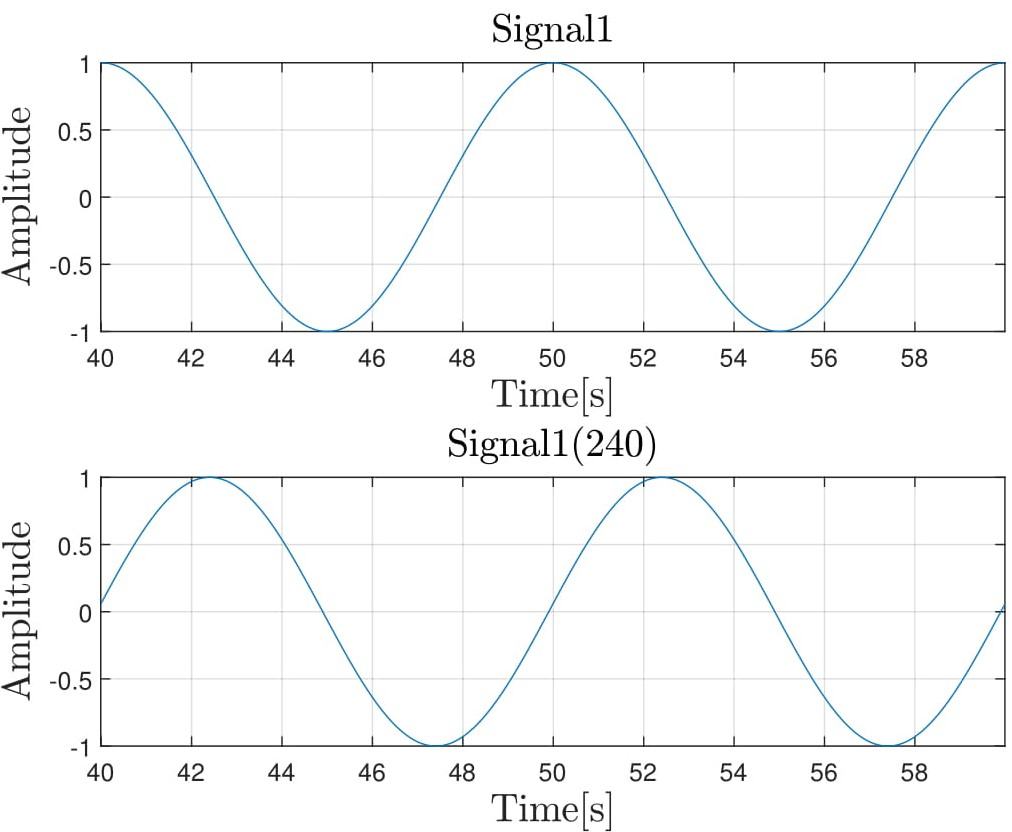
\includegraphics[width=0.8\textwidth]{Illustrations/source1.jpg}
	\caption{First Source}
	\label{fig:source1}
\end{figure}

Figure \ref{fig:source1} shows a simple sine wave. Signal1 is the original signal. 
Signal1(240) is the same signal just shifted to the right by 240 samples.
\newpage

Figure \ref{fig:source2} shows another sine wave, with a higher frequency and a 
lower amplitude. This represents another signal. Signal2 is the original signal. 
Signal2(-377) is the same signal shifted to the left by 377 samples.

\begin{figure}[htp]
	\centering
	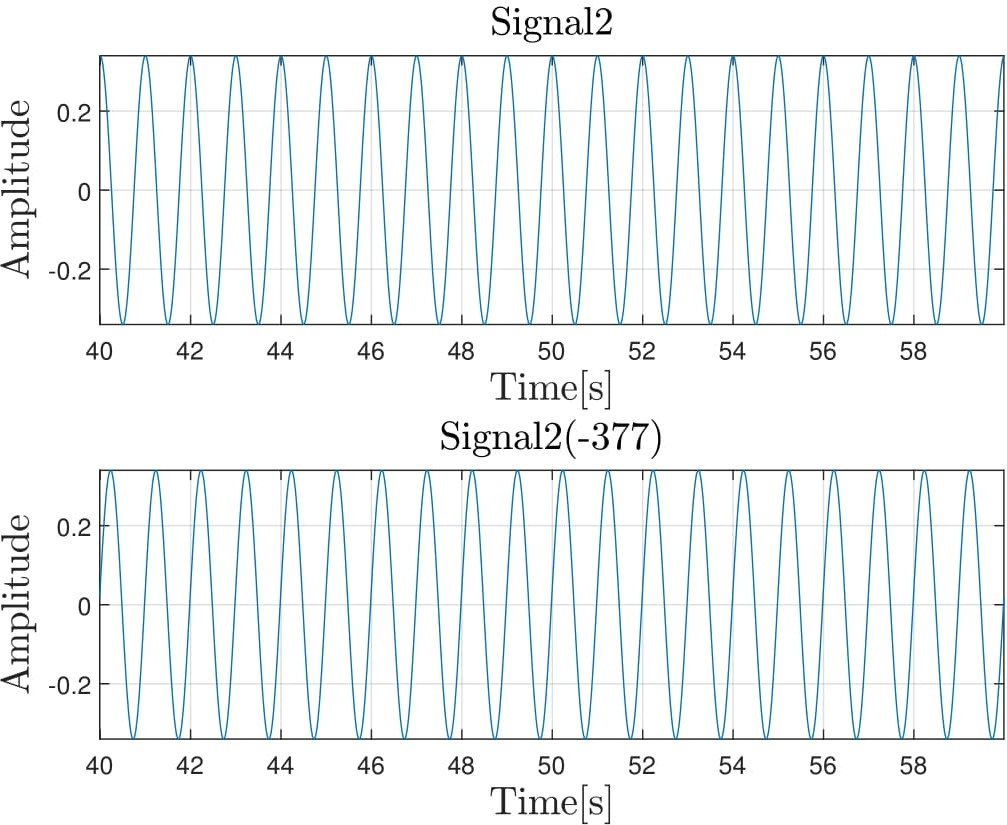
\includegraphics[width=\textwidth]{Illustrations/source2.jpg}
	\caption{Second Source}
	\label{fig:source2}
\end{figure}
Next step involves adding the signals.
\begin{equation}
	Signal1 + Signal2(-377) = LeftMicrophoneSignal
	\label{eq:leftMicrophone}
\end{equation}

\begin{equation}
	Signal1(240) + Signal2 = RightMicrophoneSignal
	\label{eq:rightMicrophone}
\end{equation}

Equations \ref{eq:leftMicrophone} and \ref{eq:rightMicrophone} now have both 
signals from both sources.
\newpage
$LeftMicrophoneSignal$ contains $Signal1$ and $Signal2(-377)$. $RightMicrophoneSignal$ contains 
$Signal1(240)$ and $Signal2$.
\begin{figure}[htp]
	\centering
	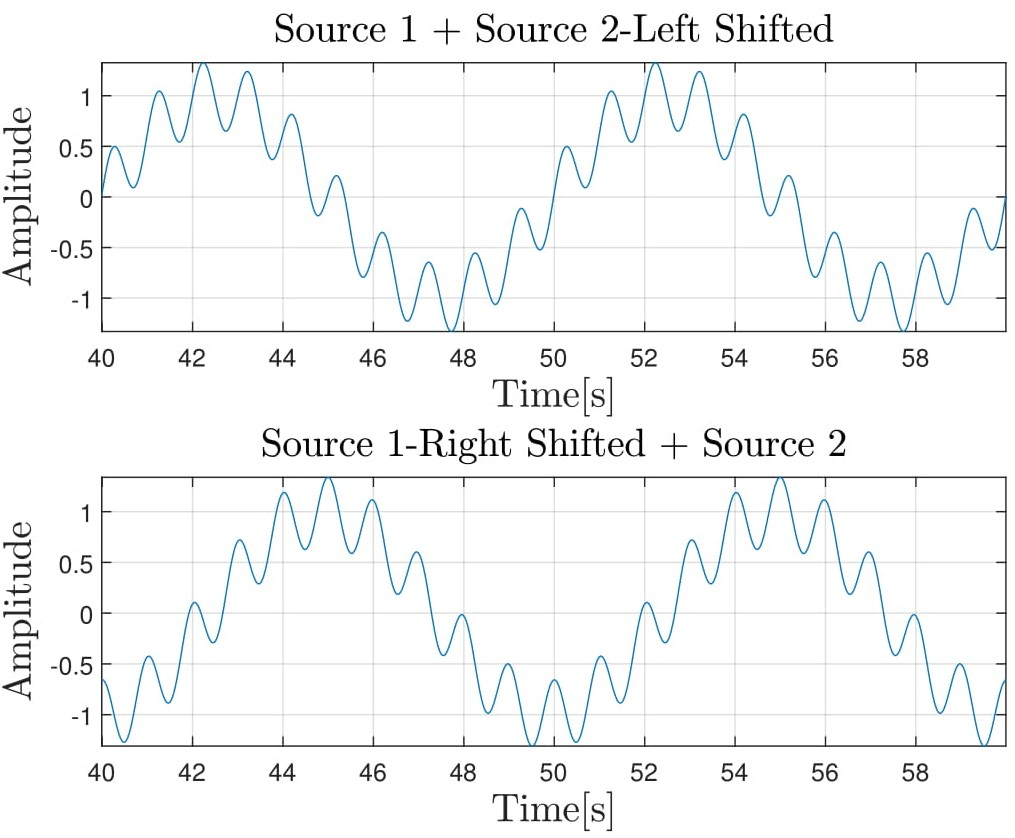
\includegraphics[width=\textwidth]{Illustrations/source1And2.jpg}
	\caption{Added Signals}
	\label{fig:source1And2}
\end{figure}

They are represented in Figure \ref{fig:source1And2}. The summation of both signals 
can clearly be seen above.
\newpage
\subsection*{Sound Separation}
We aim at separating the sounds by only using the previous signals seen in Figure 
\ref{fig:source1And2}. Knowing the angles and the amount of delay in samples, the 
separation of the two signals reduces to a matter of matching and subtracting them. 
\\
Important to notice. The matched signal is the one filtered out.\\

As stated previously, we have chosen to only shift one signal for simplicity. 
Meaning, no matter what Signal we are trying to separate, we are either going to 
shift LeftMicrophoneSignal or RightMicrophoneSignal. We have chosen to shift 
LeftMicrophoneSignal.

Suppose we are trying to get Signal2 separated.\\
First step is to match Signal1. Signal1 is part of LeftMicrophoneSignal, meaning 
LeftMicrophoneSignal has to be shifted by the same amount of samples as 
Signal1(240) in the opposite direction. That is LeftMicrophoneSignal becomes 
LeftMicrophoneSignal1(-240).\\

Next step, simply involves subtracting the two microphone signals as shown in 
Equation \ref{eq:obtainedSignal1}.

\begin{equation}
	LeftMicrophoneSignal(-240) - RightMicrophoneSignal = ObtainedSignal1
	\label{eq:obtainedSignal1}
\end{equation}

Similarly, Signal2 can be obtained, as shown in Equation \ref{eq:obtainedSignal2}.

\begin{equation}
	LeftMicrophoneSignal(377) - RightMicrophoneSignal = ObtainedSignal2
	\label{eq:obtainedSignal2}
\end{equation}
\newpage
Figure \ref{fig:obtainedSignals} represents the obtained signals after matching and 
subtracting the signals in figure \ref{fig:source1And2}.

\begin{figure}[htp]
	\centering
	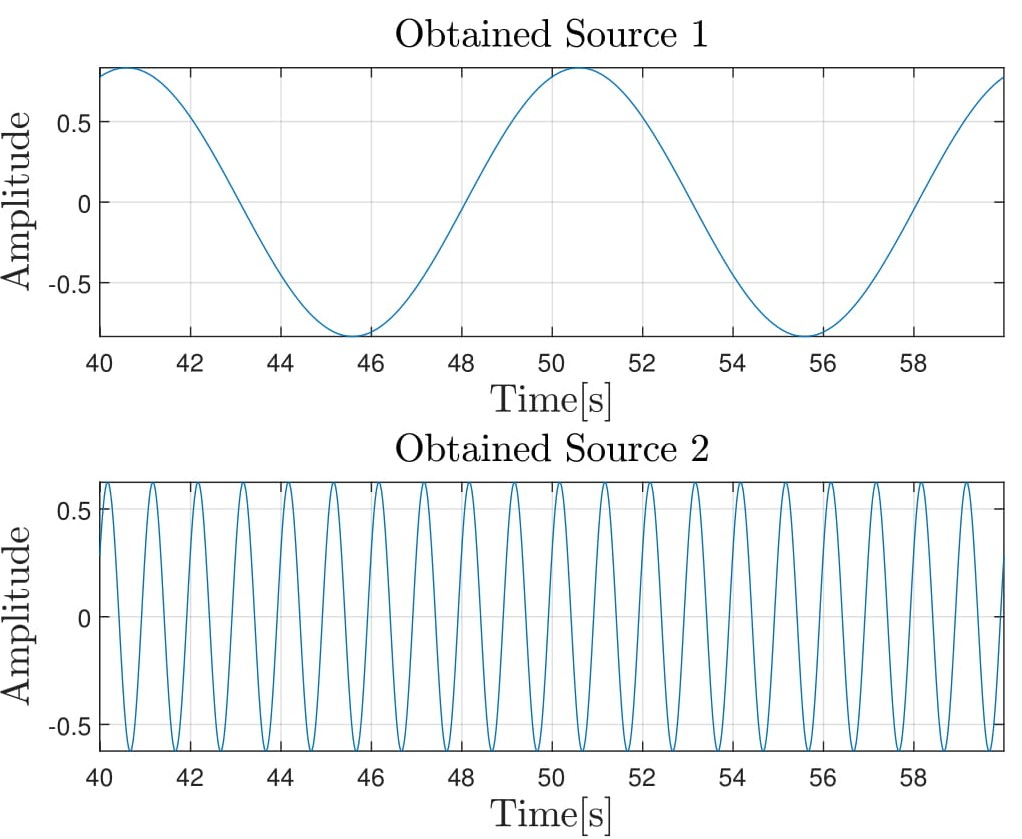
\includegraphics[width=\textwidth]{Illustrations/obtainedSource1And2.jpg}
	\caption{Obtained Signals}
	\label{fig:obtainedSignals}
\end{figure}

The waveforms of the signals are similar. However, there seems to be a slight amplitude 
increase, which we believe has something to do with the way we are filtering. Although the
waveforms we are filtering look similar, they have different amplitudes, due to the way
they would be recorded. Meaning, we either get a lower or a higher amplitude. Depending on
where the sound comes from.

\newpage
\section{Filtering}
All of the directional filtering is done by applying the logic discussed before. 
Prior to shifting signals and do the actual filtering, we had to remove any other 
delays, introduced by hardware and software.

We attempted to resolve this issue by introducing a loud sound, such as a finger 
snap, or a clap at the start of every recording session. Using that, we matched the 
highest peaks, and eliminated a big part of the delay caused by anything else 
besides the distance between the microphones.

\subsection{One Source}
Initially, a recording by only one person sitting in the center, meaning 0$^\circ$, 
was recorded, to observe if after all the other delays were eliminated, the data 
would match.\\

Figure \ref{fig:C} represents the data collected. As can be observed on the figure, 
the two signals match in phase, and have fairly similar amplitudes.
\begin{figure}[htp]
  \centering
  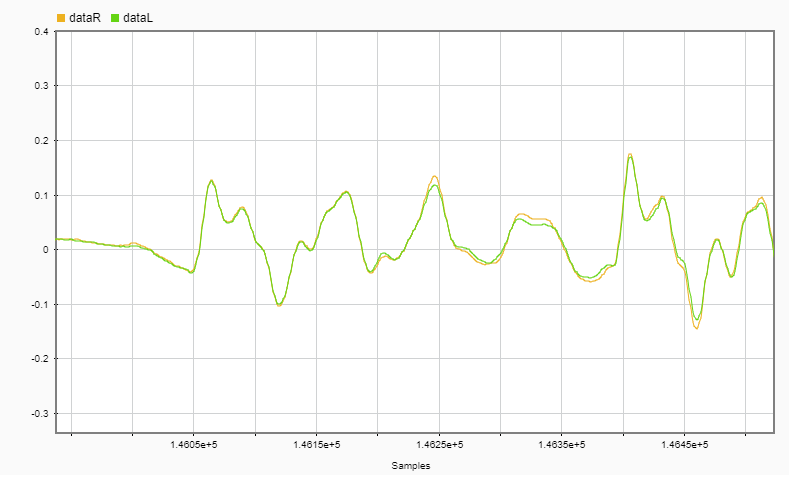
\includegraphics[width=0.8\linewidth]{Illustrations/DataC.png}
  \caption{Center Sound Source}
  \label{fig:C}
\end{figure}

\newpage

When recording with the sound source coming from the right of the setup, the right 
microphone has slightly higher amplitude and its' data leads the left microphone 
data as seen in Figure \ref{fig:R}.

\begin{figure}[htp]
  \centering
  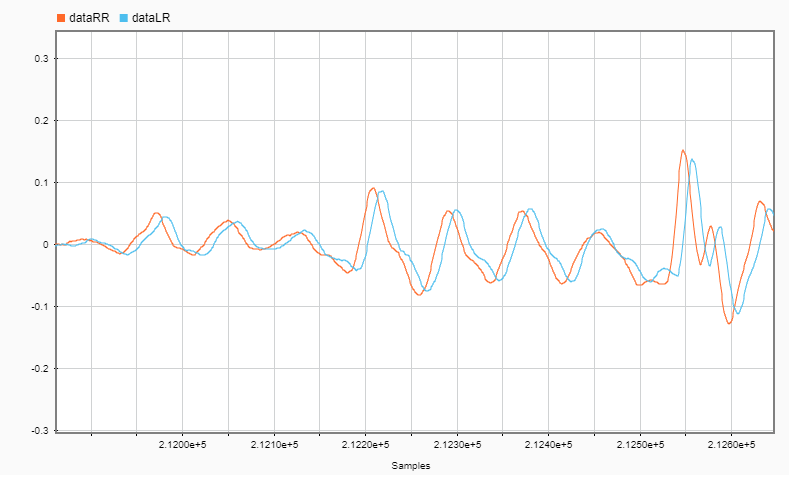
\includegraphics[width=0.8\linewidth]{Illustrations/DataR.png}
  \caption{Right Sound Source}
  \label{fig:R}
\end{figure}

Another recording was taken, this time with a sound source coming from the left. 
The results can be seen in Figure \ref{fig:L}.

\begin{figure}[htp]
  \centering
  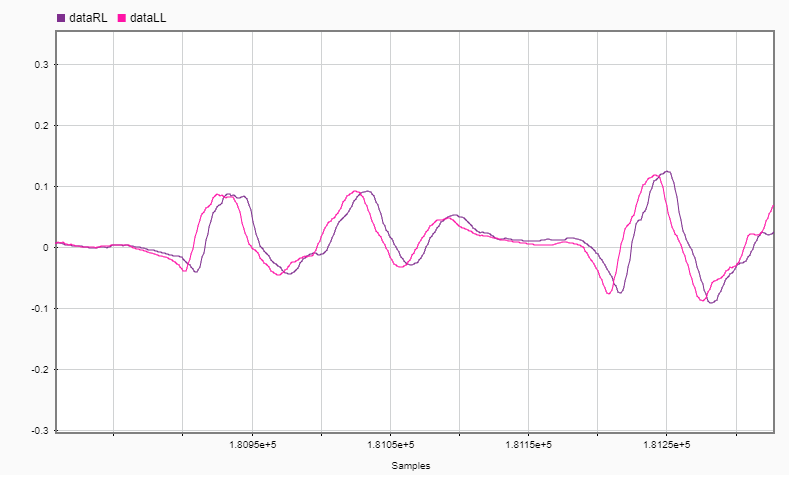
\includegraphics[width=0.8\linewidth]{Illustrations/DataL.png}
  \caption{Left Sound Source}
  \label{fig:L}
\end{figure}

\newpage
\subsection*{Results}
An early attempt at filtering speech, was done on only one person. The data was 
firstly matched, and then subtracted. The result of it, can be seen in Figure 
\ref{fig:oneSourceSepAndOG}. 
The green data represents the original recorded 
signal, while the blue data represents the separated data. Ideally, the blue data 
would have very low amplitude, and should be inaudible.

However, after listening to the signal, it still contained enough data to hear what 
the person that should be filtered out, is saying. Even though the goal was 
relative silence, the sound level dropped significantly.

\begin{figure}[htp]
  \centering
  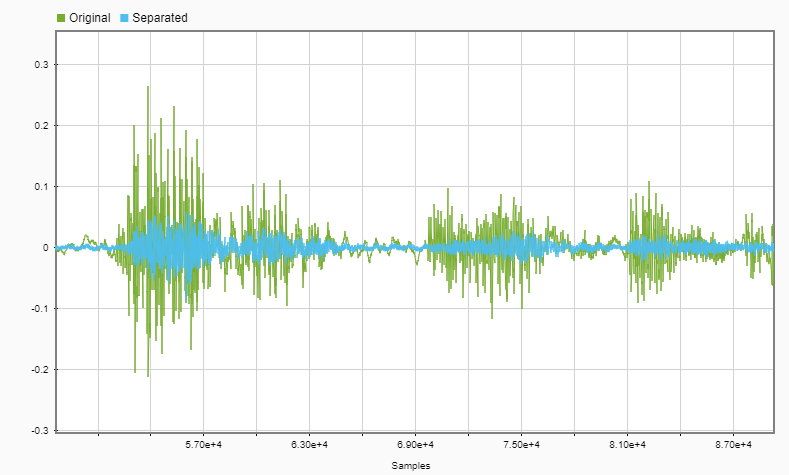
\includegraphics[width=\linewidth]{Illustrations/OnePersonOriginalAndSeparated.png}
  \caption{Data Comparison One Source}
  \label{fig:oneSourceSepAndOG}
\end{figure}

\newpage

\subsection{Two Sources}
The same separation method was applied for two sources. Due to no other sounds 
being present, we assumed that this might be one of the reasons we were able to 
still hear some of the original speech that was intended to be filtered out. If 
other sound would be present, maybe their strength would overcome the signal that 
was intended to be filtered out.\\

After shifting the left microphone data, some data lines up with the right 
microphone data, which can be observed in the green square in Figure \ref{fig:2sourcesShifted}, 
which suggests it could work and it would separate the unwanted sounds from the samples. 

\begin{figure}[htp]
  \centering
  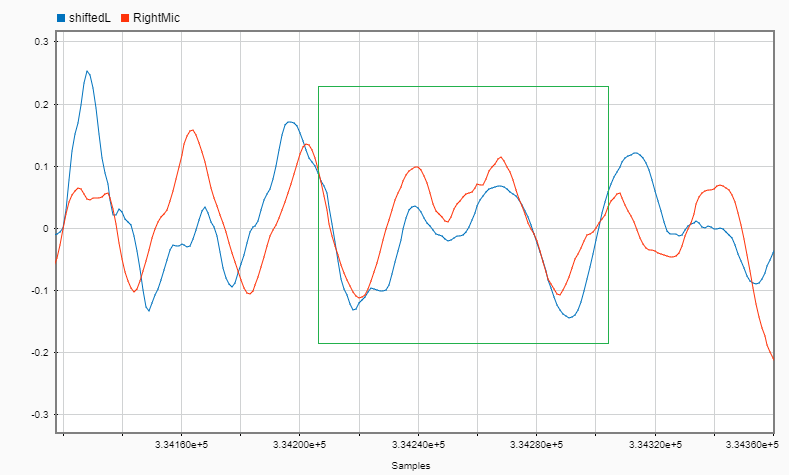
\includegraphics[width=1\linewidth]{Illustrations/twoSourcesShiftedandOriginal.png}
  \caption{Two Sources, Aligned Data}
  \label{fig:2sourcesShifted}
\end{figure}
\newpage
The separated data was compared to the original data. The comparison can be seen in figure \ref{fig:2sourcesSeparated}.
\begin{figure}[htp]
  \centering
  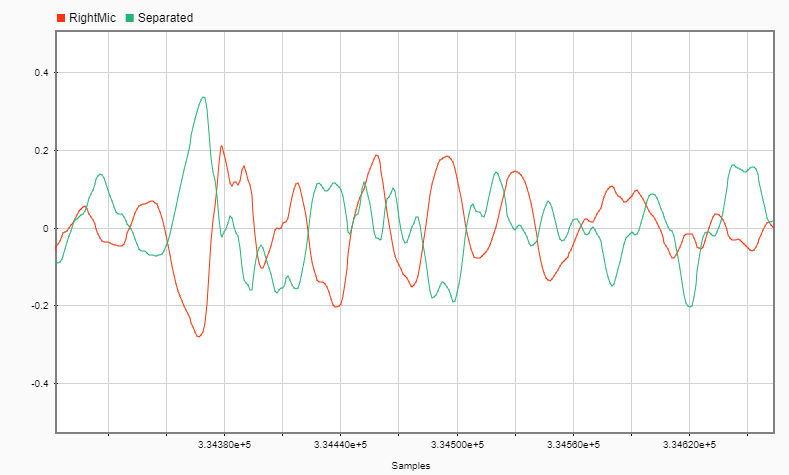
\includegraphics[width=0.7\linewidth]{Illustrations/twoSourcesSeparatedandOriginal.png}
  \caption{Separated Signal And Original Signal}
  \label{fig:2sourcesSeparated}
\end{figure}

Idealy, the two waveforms above would look the same, or at least similar. However
no resemblance can be seen, suggesting the sound separation did not work as 
expected.

\subsection*{Results}

This was deemed as a failed attempt. However not necessarily because of the method, 
but rather because of the, equipment used and environment to record the samples, 
which were not ideal. Neither of the microphones captured the sound waves 
identically. This can be seen in Figure \ref{fig:clap}. The clap at the beginning 
of the recordings can be represented. Ideally, microphones would register identical 
waveform, but in the figure they are clearly different.\\


\begin{figure}[htp]
  \centering
  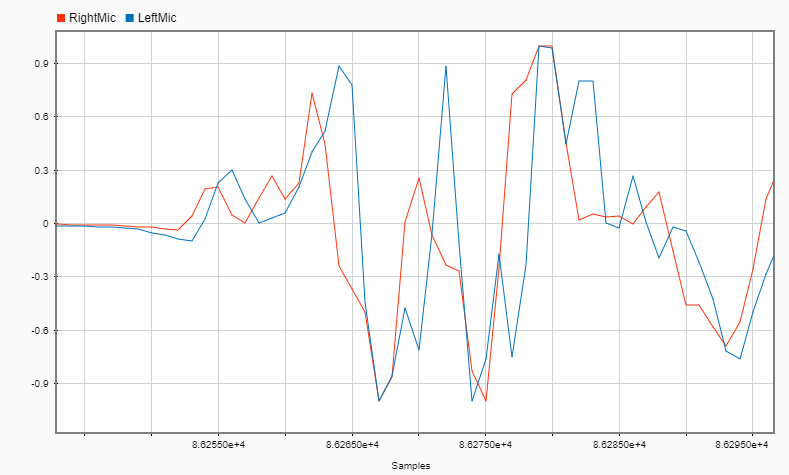
\includegraphics[width=0.7\linewidth]{Illustrations/clap.png}
  \caption{Clap Waveform}
  \label{fig:clap}
\end{figure}
\newpage

\section{Synthetic Samples}
Failing to observe any noticeable separation when using real samples, we have 
decided to attempt the same separation method using synthetic samples. This was 
done in order to find out if the method was in itself wrong, or something else had 
a bigger impact, due to which we were unable to see any differences. Synthetic 
samples were made, by recording one person talking, and then articulating the data 
to take delay and gain into account, in an attempt to make them sound as real as 
possible.\\


Using synthetic samples also allowed for more flexibility when testing the code, by 
being able to adjust the angle of the source. 

\subsection*{Gain ratio}
A gain needs to be multiplied with one of the signals, to account for the distance 
difference. If one source is closer to one microphone than the other, the signal 
from that source needs to have a higher strength, to mimic real behavior of the 
scenario. \cite{GAIN}

Sound strength falls by a ratio of 0.5 when the distance is doubled. Meaning that 
sound strength follows distance inverse-proportionally.
 
By giving one of the microphones gain ratio of 1, the ratio for the other signal 
can be determined. Figure \ref{fig:ratioDependence} illustrates the variables used 
in the equations.

\begin{figure}[htp]
	\centering
	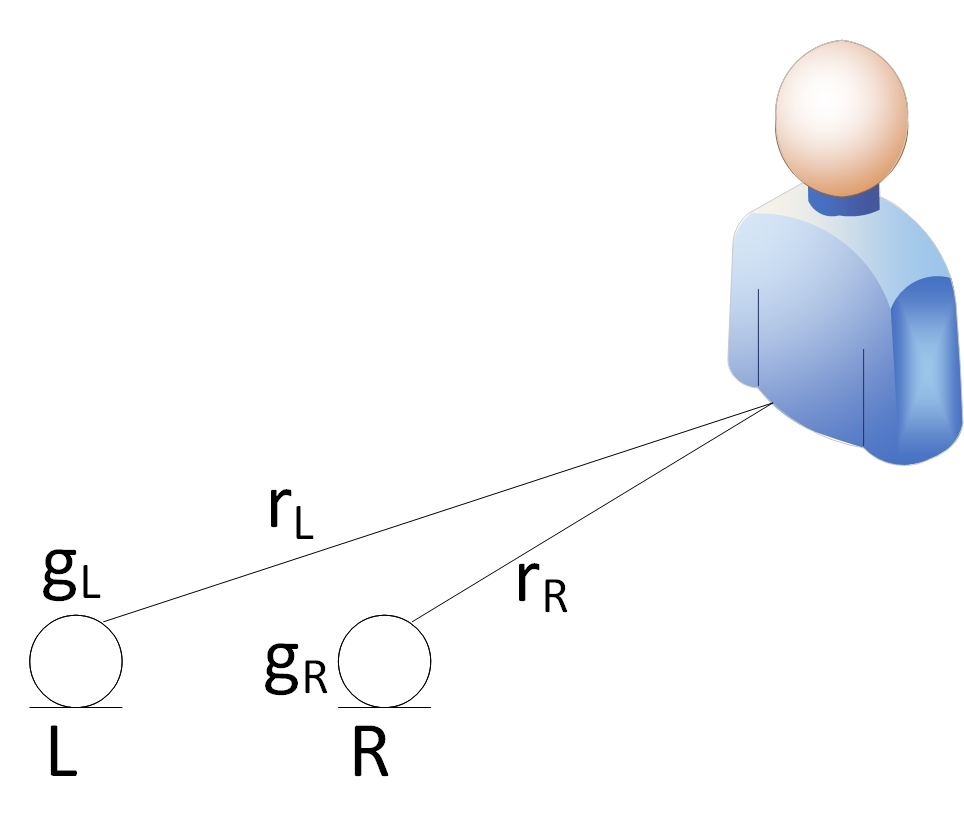
\includegraphics[width=0.35\textwidth]{Illustrations/gainRatio.jpg}
	\caption{Gain Ratio}
	\label{fig:ratioDependence}
\end{figure}

\begin{equation}
	\frac{r_L}{r_R} = \frac{dist_R}{dist_L}
\end{equation}
\begin{equation*}
	r_L = LeftMicrophoneSignalGain
\end{equation*}
\begin{equation*}
	r_R = RightMicrophoneSignalGain
\end{equation*}
\begin{equation*}
	dist_L = SourceToLeftMicrophoneDistance
\end{equation*}
\begin{equation*}
	dist_R = SourceToRightMicrophoneDistance
\end{equation*}
\newpage
Using this proportion and keeping \(r_L\) as 1, the gain \(r_R\) will be multiplied 
with right microphone data to get realistic gain loss. Distances \(dist_L\) and 
\(dist_R\) here are the same distances, which are calculate in the delay code. This 
means that in order to get the gain ratio for right microphone, the distance to the 
left microphone (\(dist_L\)) needs to be divided by distance to the right 
microphone (\(dist_R\)).

\subsection*{Adding recordings}
Firstly, each recording is shifted by an amount of samples, corresponding to the 
angle we want. Afterwards, they are multiplied by their respective gains. Lastly, 
they are cut down to the same size to make the adding easier. RightMicrophoneSignal 
corresponding to each source will be multiplied by the gain, while LeftMicrophoneSignal  
corresponding to each source will be shifted. Figure \ref{fig:SplitTwoSources} 
visualizes how two summed signals look like. The figure represents a split view of
the added signals. Each signal is a sum of two other signals, shifted and multiplied
by a specific gain. To the right of the red line, each signal is only comprised of
one signal, to represent the matching of the signals. A slight delay is noticed
and a difference of amplitude. 

\begin{figure}[htp]
	\centering
	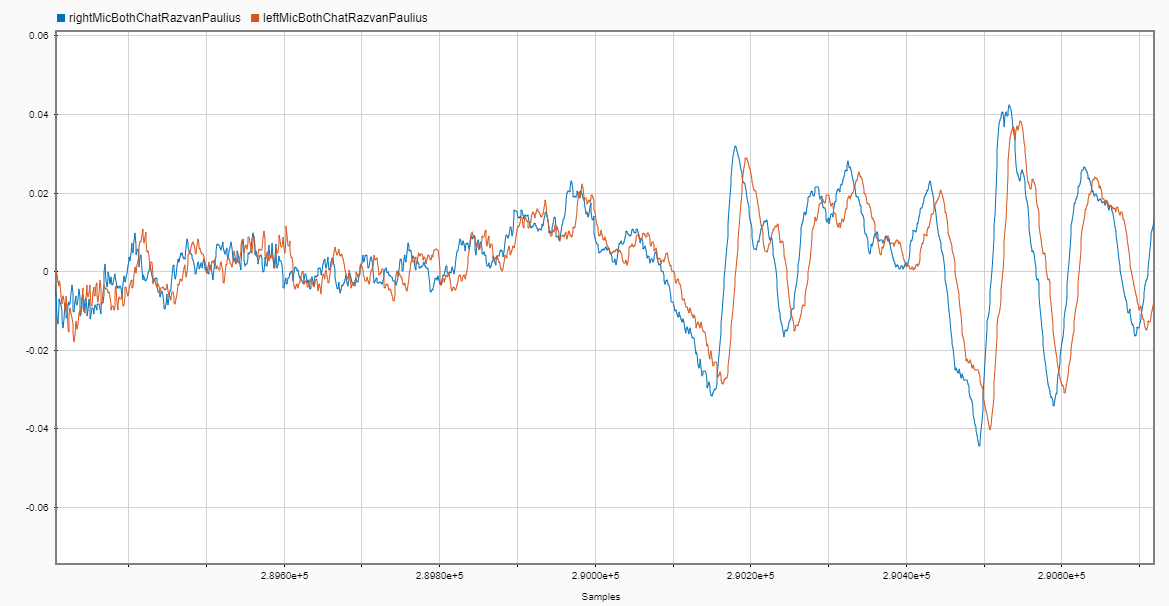
\includegraphics[width=.9\textwidth]{Illustrations/twoSourcesAndJustOneLater.png}
	\caption{Split View of Signals}
	\label{fig:SplitTwoSources}
\end{figure}
\newpage
Further on, LeftMicrophoneData has to be shifted to match the phase of RightMicrophoneData.
The results can be seen in Figure \ref{fig:SplitShifted}.
\begin{figure}[htp]
	\centering
	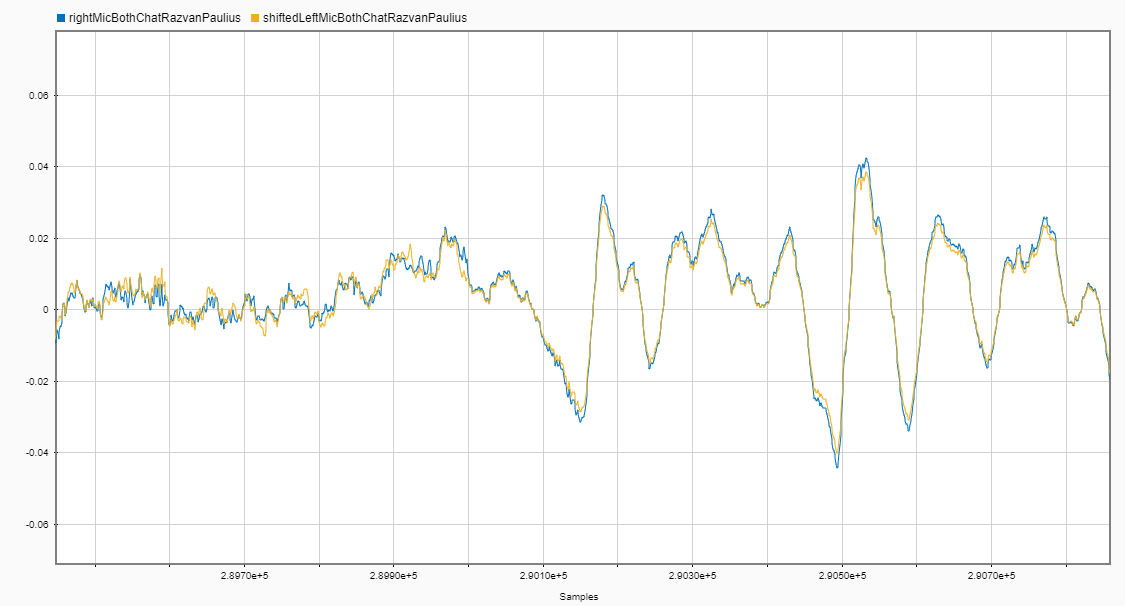
\includegraphics[width=.8\textwidth]{Illustrations/shiftedLeftAndRightSplitView.png}
	\caption{Split View of Shifted Signals}
	\label{fig:SplitShifted}
\end{figure}

After separating the signals, the result can be seen in Figure \ref{fig:SplitSeparated}.
Notice that the green signal nears zero to the right of the red line. To the left of the
red line, the signal has a different waveform, suggesting the matched signal has been
separated, and only the other signal is left.

\begin{figure}[htp]
	\centering
	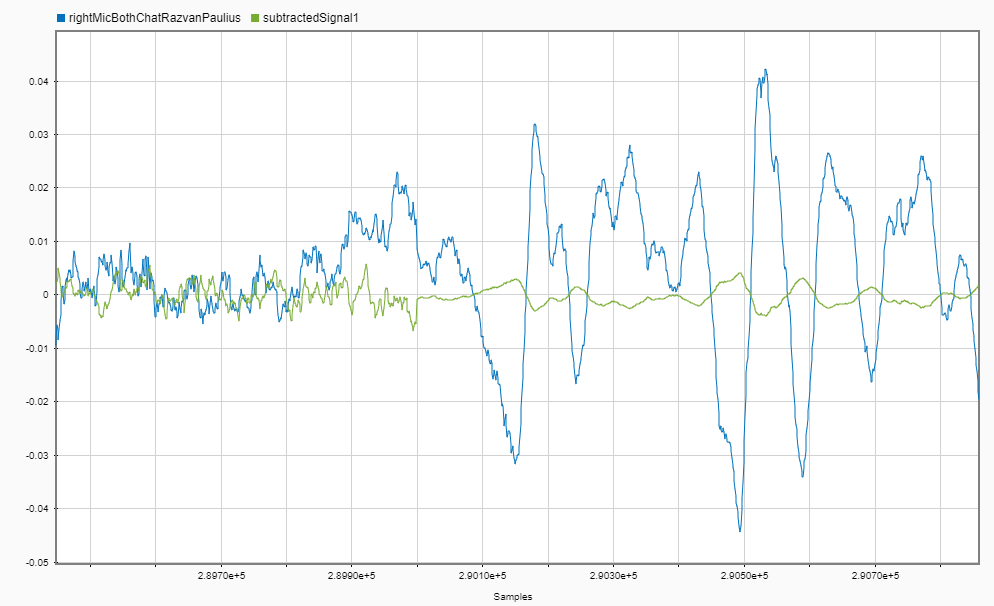
\includegraphics[width=.8\textwidth]{Illustrations/rightAndSubtractedSplitView.png}
	\caption{Split View of Subtracted Signal}
	\label{fig:SplitSeparated}
\end{figure}




\newpage
\subsection*{Results} 
The speech separation was attempted successfully with synthetic samples. Either of 
the sources can be separated and clearly heard. The filtering method however, has 
some limitations. If the angle between the sources is too big, the gains of each 
signals are significant enough to not be able to filter them out completely just 
by subtracting. We are hoping that by using machine learning, this issue could be 
solved as well.